\subsection{20 августа. пер. Уллукёль Восточный (1А*)}
\textit{Метеоусловия: утром, днём ясно, вечером~--- переменная облачность, тепло.}

\begin{figure}[h!]
	\centering
	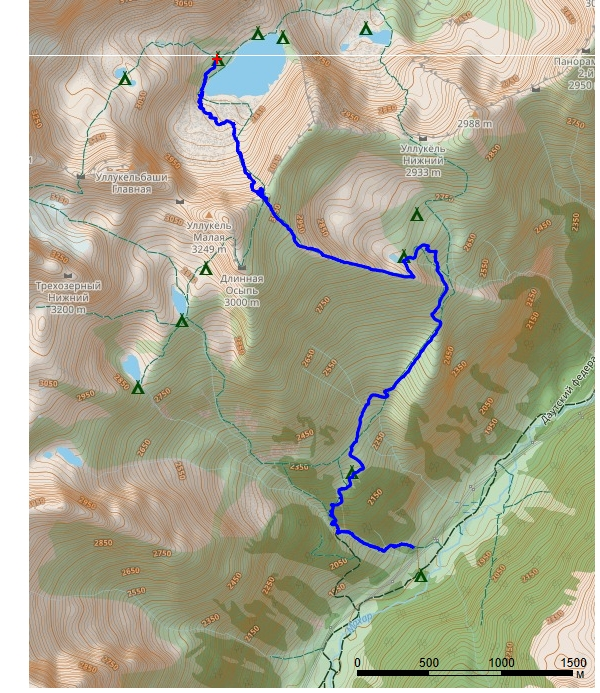
\includegraphics[angle=0, width=0.7\linewidth]{../pics/mini_maps/20}
	\label{fig:mini_20}
\end{figure}

Подъём дежурных в 04:30, общий подъём в 05:00. Выход группы в 07:30 (рис.~\ref{fig:20aug1.jpg}).

\begin{figure}[h!]
	\centering
	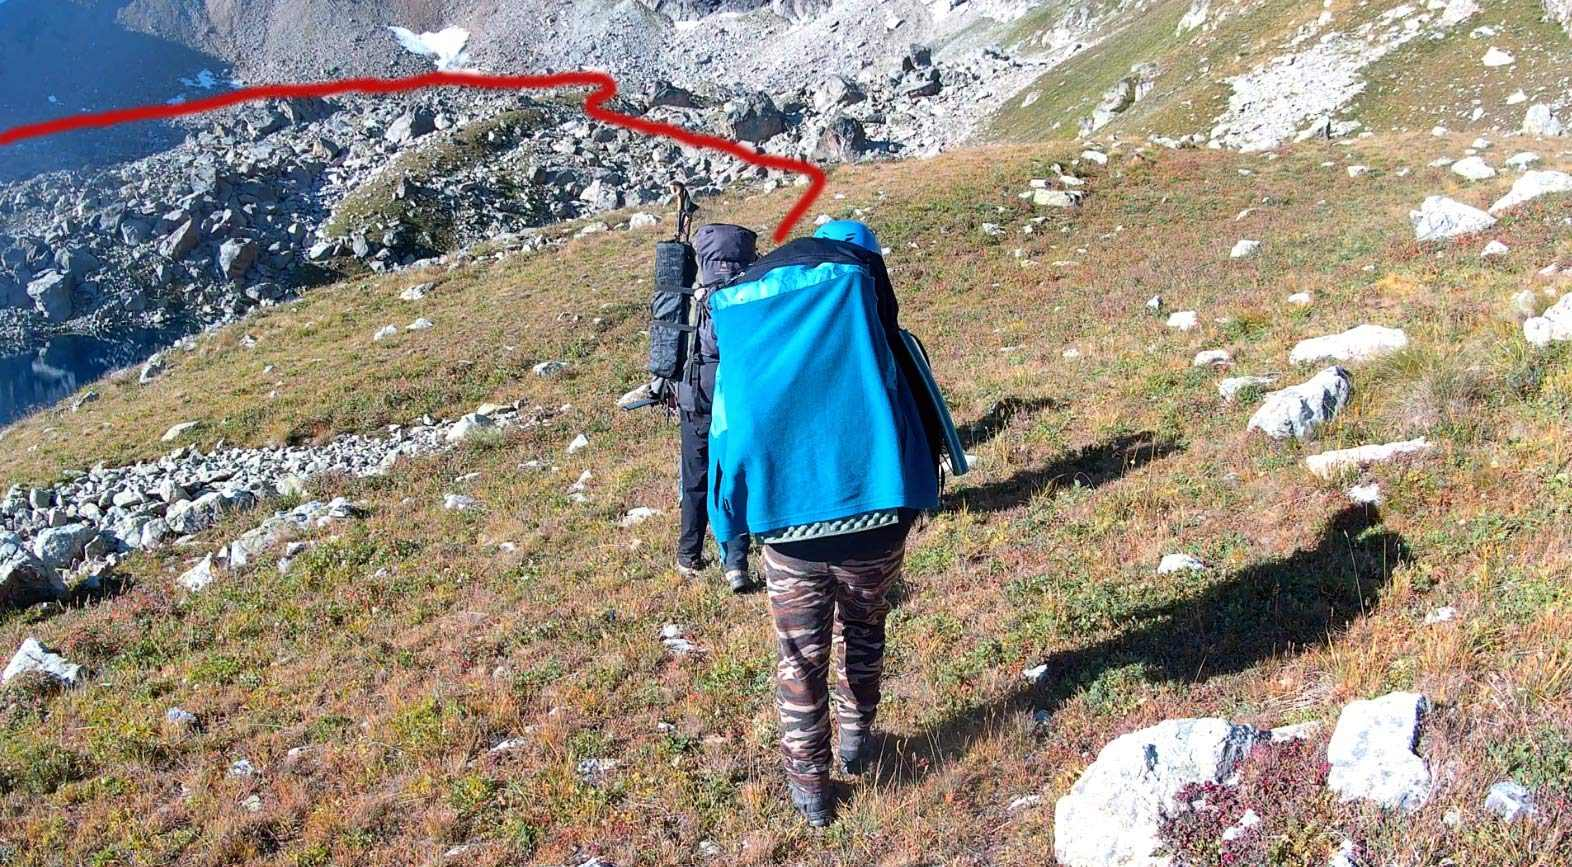
\includegraphics[width=0.7\linewidth]{../pics/20aug1.jpg}
	\caption{Подход под перевал от м.н.}
	\label{fig:20aug1.jpg}
\end{figure}


 Движемся по разведанному вчера маршруту по крупной осыпи в обход южной оконечности озера. На одном из привалов участнице (Наташе Мироновой) становится нехорошо, и часть пути (ок. 15 мин. ЧХВ) она проходит без рюкзака. Пока доносим рюкзак, группа фотографируется на фоне озера на небольшом зелёном гребешке (рис.~\ref{fig:DSC_0907}).
 
 \begin{figure}[h!]
 	\centering
 	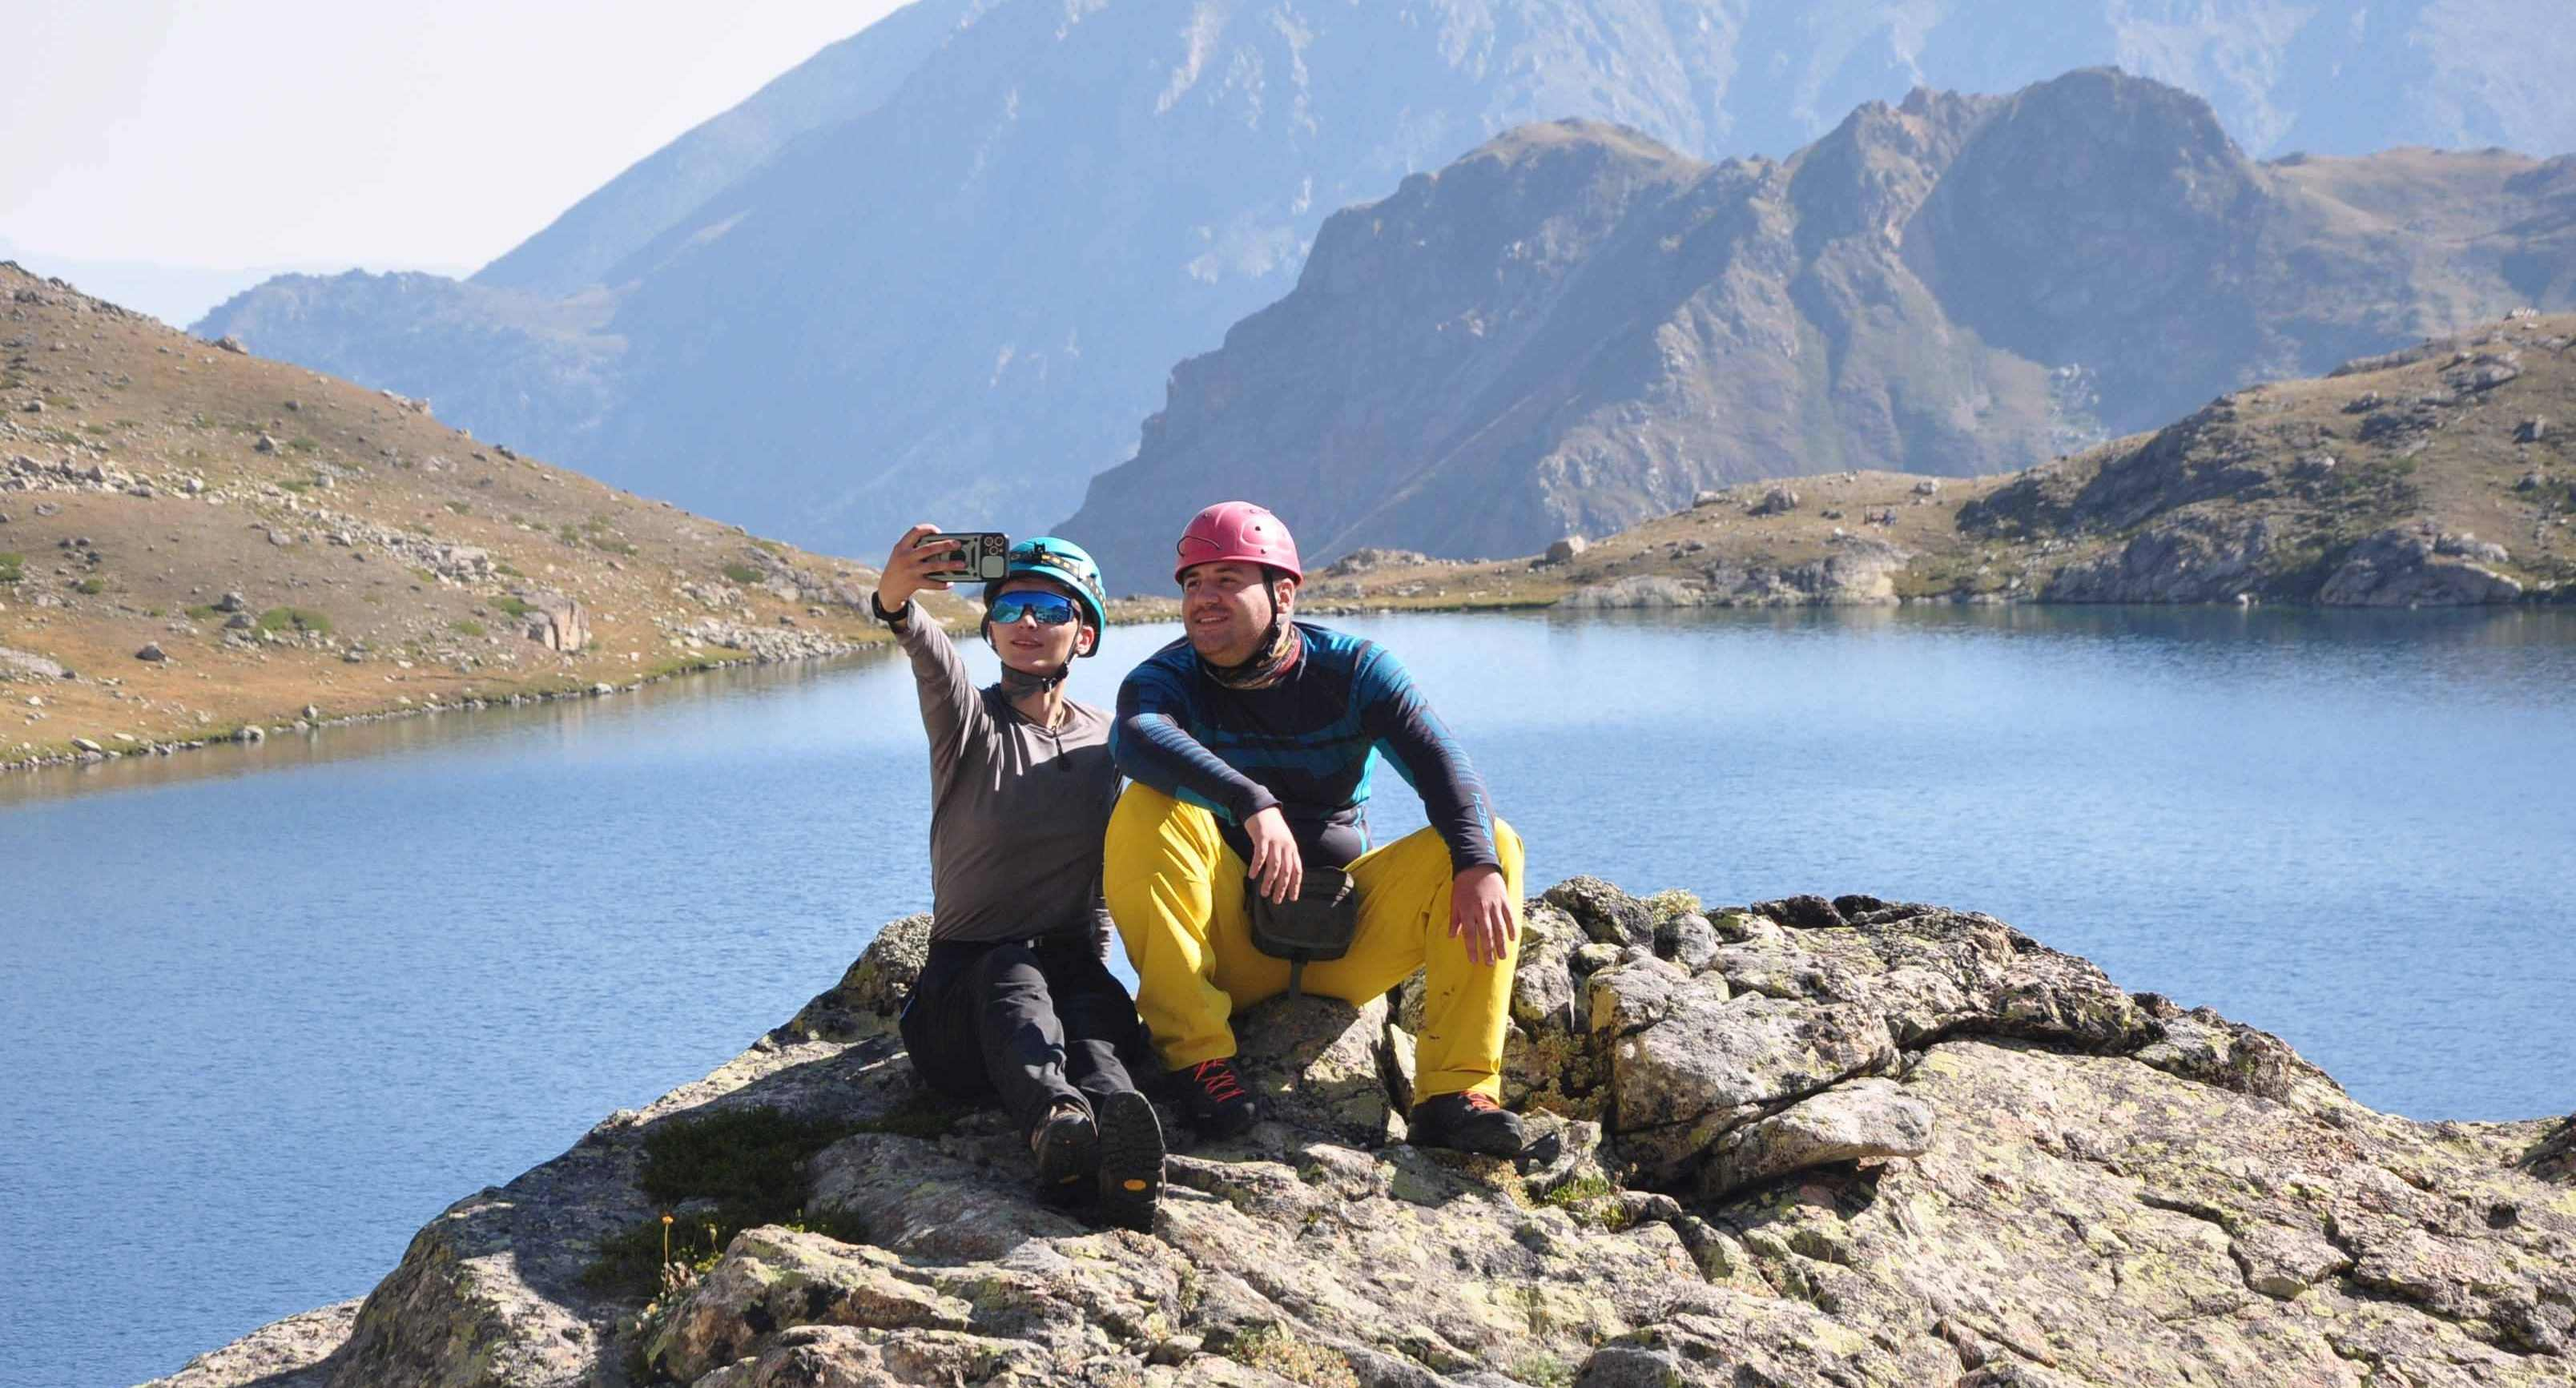
\includegraphics[width=0.7\linewidth]{../pics/DSC_0907}
 	\caption{Фоткаемся на фоне озера}
 	\label{fig:DSC_0907}
 \end{figure}
 

Далее движемся на юго-восток по морене до другого зелёного гребешка, ведущего под перевальный взлёт (рис.~\ref{fig:20aug2.jpg}) и в 9:40 выходим на среднюю осыпь перевального взлёта, прижимаясь к правому пхд борту кулуара.

\begin{figure}[h!]
	\centering
	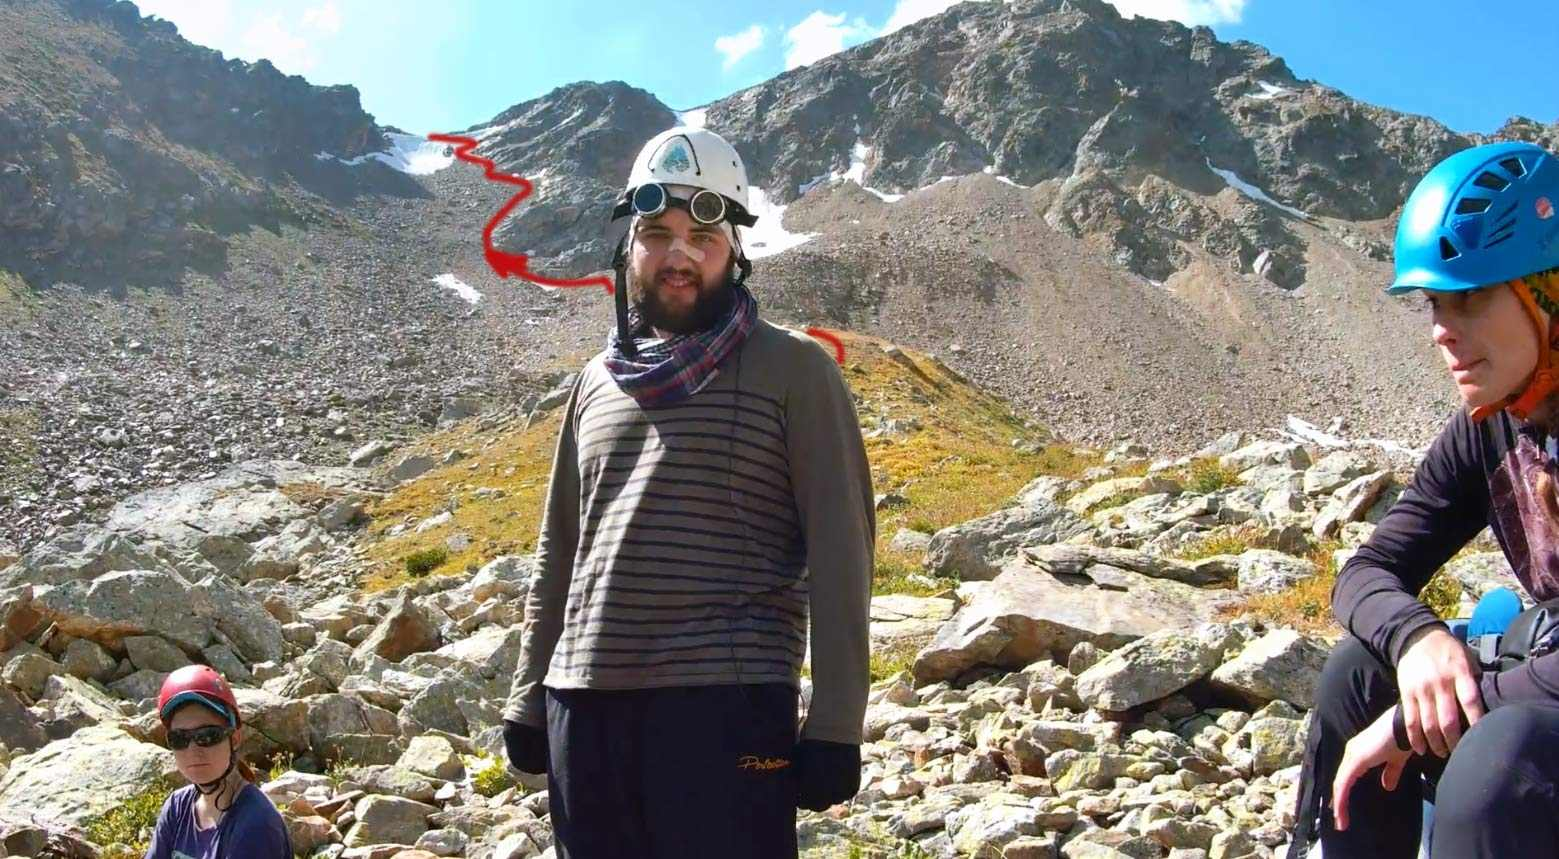
\includegraphics[width=0.7\linewidth]{../pics/20aug2.jpg}
	\caption{Маршрут движения по перевальному взлёту}
	\label{fig:20aug2.jpg}
\end{figure}

Снега на перевальном взлёте почти нет, поэтому руководитель принимает решение двигаться не по линии падения воды, а по правому борту кулуара. Осыпь местами живая, движемся не спеша. В 12:25 достигаем полочки, на уровне которой начинается самая крутая часть перевального взлёта и снежник. Надеваем кошки и движемся косым траверсом влево пхд, чтобы выйти на седловину. Снег мягкий, возможно организовывать ступени, если ставить ногу на всю ступню. На седловине снежного карниза нет, но присутствует удобный снежный карман (рис.~\ref{fig:DSC_0946}). За 70 м тропёжки произвели две смены лидера.

\begin{figure}[h!]
	\centering
	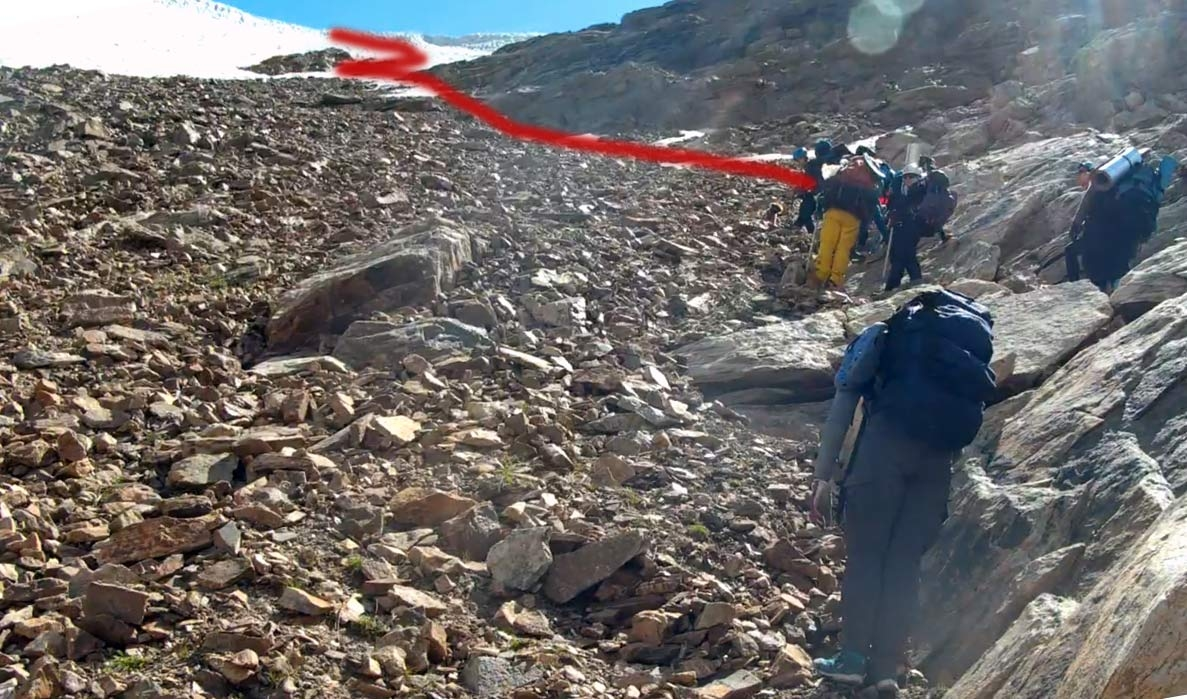
\includegraphics[width=0.7\linewidth]{../pics/20aug3.jpg}
	\caption{Движение по правому пхд борту кулуара}
	\label{fig:20aug3.jpg}
\end{figure}

\begin{figure}[h!]
	\centering
	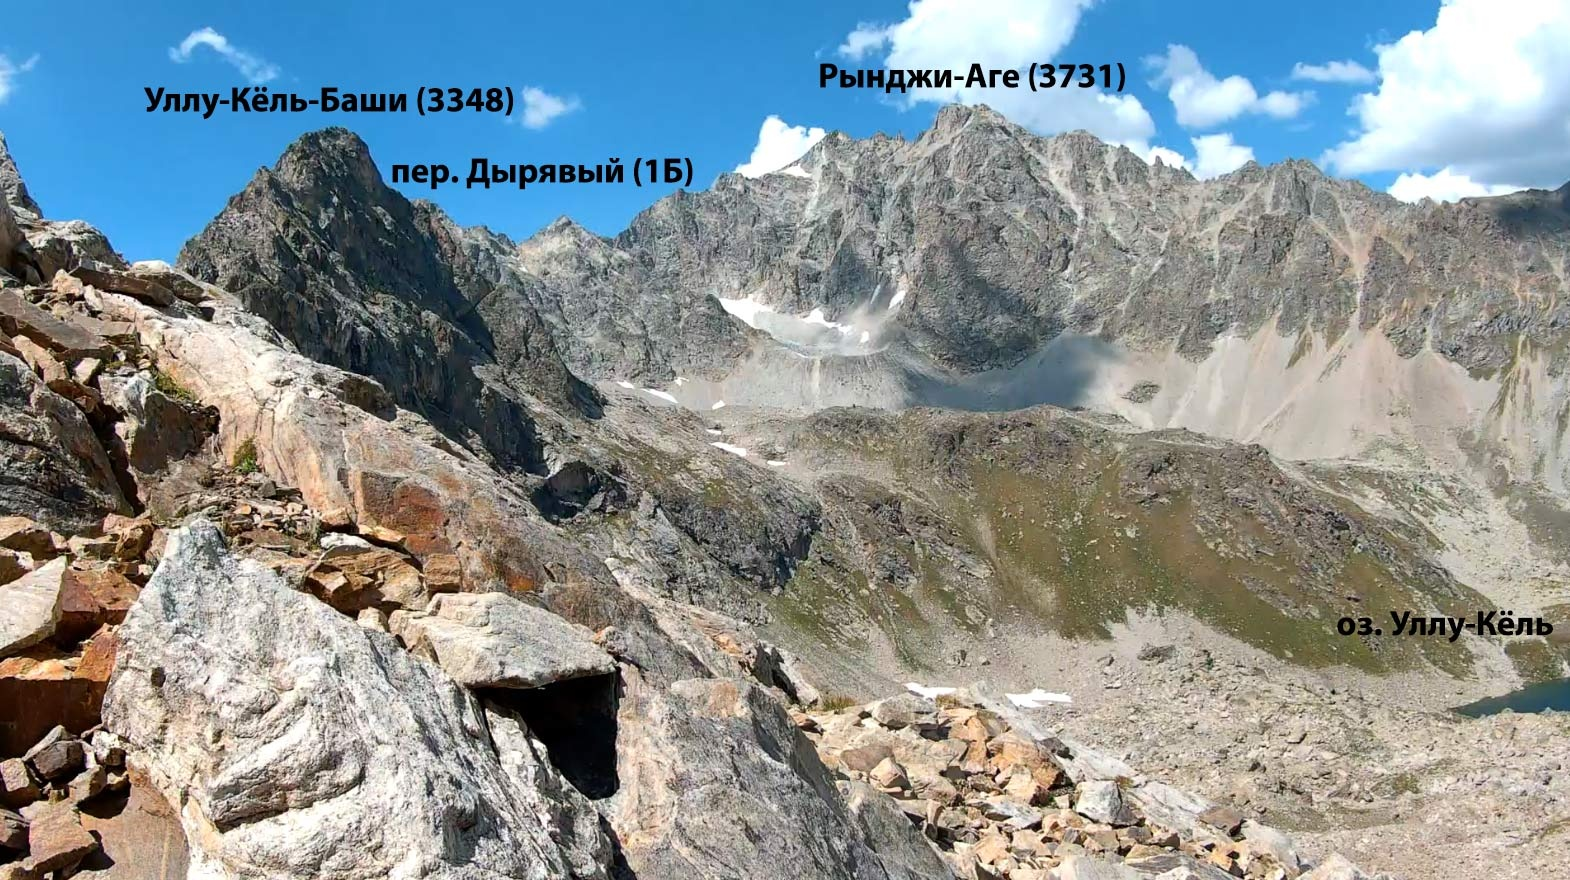
\includegraphics[width=0.7\linewidth]{../pics/20aug4.jpg}
	\caption{Вершины и перевалы цирка Уллу-Кёль}
	\label{fig:20aug4.jpg}
\end{figure}

%Когда до снежного кармана (безопасной зоны) оставалось около 3 м по вертикали, лидер, Катя Тюрина, срывается \remove{из-за того, что собаку на руки взяла}. Пролетев  50 метров по снежному склону крутизной 45\degree, Катя не успевает окончательно зарубиться и останавливается только на осыпном склоне, перекувыркнушись через голову



Группа встала в районе 5:30, вышла в 7:29. Погода была солнечной и теплой, облаков не было. На момент выхода у нас в группе было 3 человека, у которых было плохое самочувствие. Решили их разгружать. Начало пути пролегало через курумник.  В 8:10 продолжали идти, один из участников с плохим самочувствием оставил рюкзак и шел без него, а второй участник, оставив свой рюкзак на привале, вернулся и принес оставленный.  После курумника начиналась сыпуха, которая весьма активно уходила из под ног. В 12: 29 начало большого привала, надеваем кошки, так как дальше шел снежник. Тропила и делала ступеньки К. В районе 13:5 (13:45) К. сорвалась. Пролетела 60 метров по снежнику, зарубившись. В конце спуска сделал сальто на камни, после чего большой камень упал на руку. Участник А провел себе осмотр на травмы, сильно не пострадал. В 13:55 остальная группа взошла на перевал, после чего руковод и зам.руководителя спустились за участником А. Участник А сам взобрался обратно на перевал без рюкзака. На самом перевале нашли записку и оставили свою.  В 15:48 вышли на спуск, участник А шел со своим рюкзаком. Спуск был по низкой траве с камнями. Путь держали по маленькому хребетику вниз к озеру.  В 16:54 обед у озера. В 18:16 вышли. Далее в 18:41 у участника Г. упала каска, разделились, в 18:55 встретились и пошли дальше. Спустившись до дома пастуха, спросили дальнейшую дорогу. Уже было темно, поэтому начали голосование, где вставать на ночевку. Было принято решение идти дальше до запланированной ночевки. 
В 22:15 встали на ночевку у реки.



\begin{figure}[h!]
	\centering
	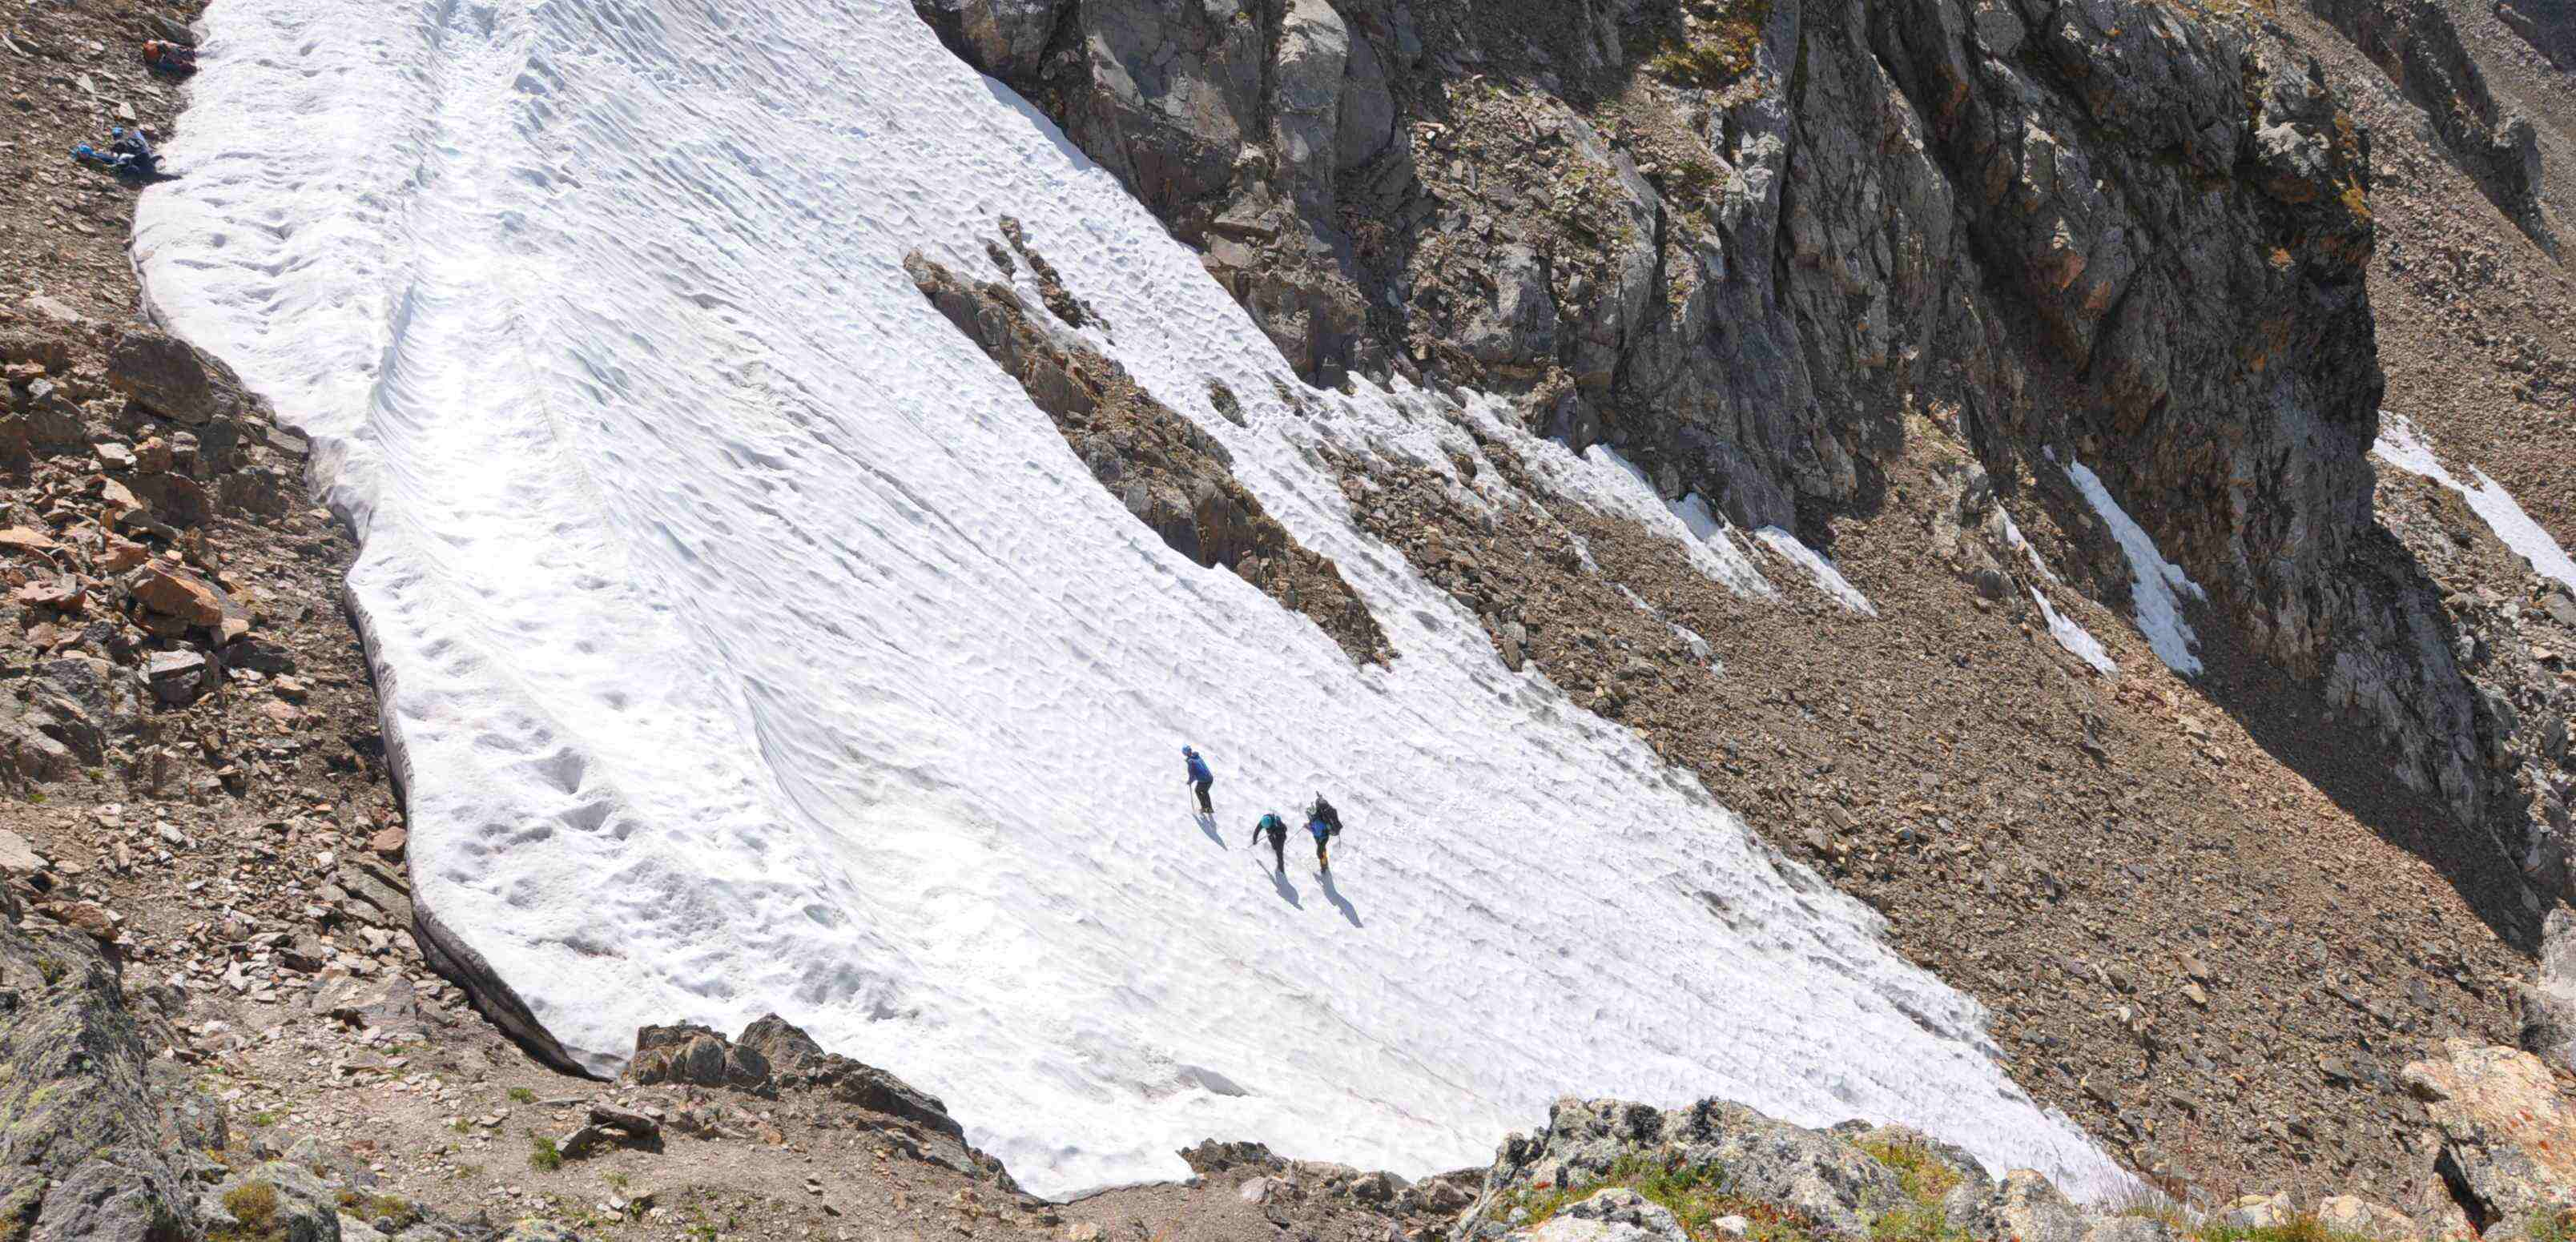
\includegraphics[width=0.7\linewidth]{../pics/DSC_0946.png}
	\caption{Маршрут движения группы по снежнику (красный), траектория срыва участника (синий), маршрут подъёма с сорвавшимся участником (чёрный)}
	\label{fig:DSC_0946}
\end{figure}


\begin{figure}[h!]
	\centering
	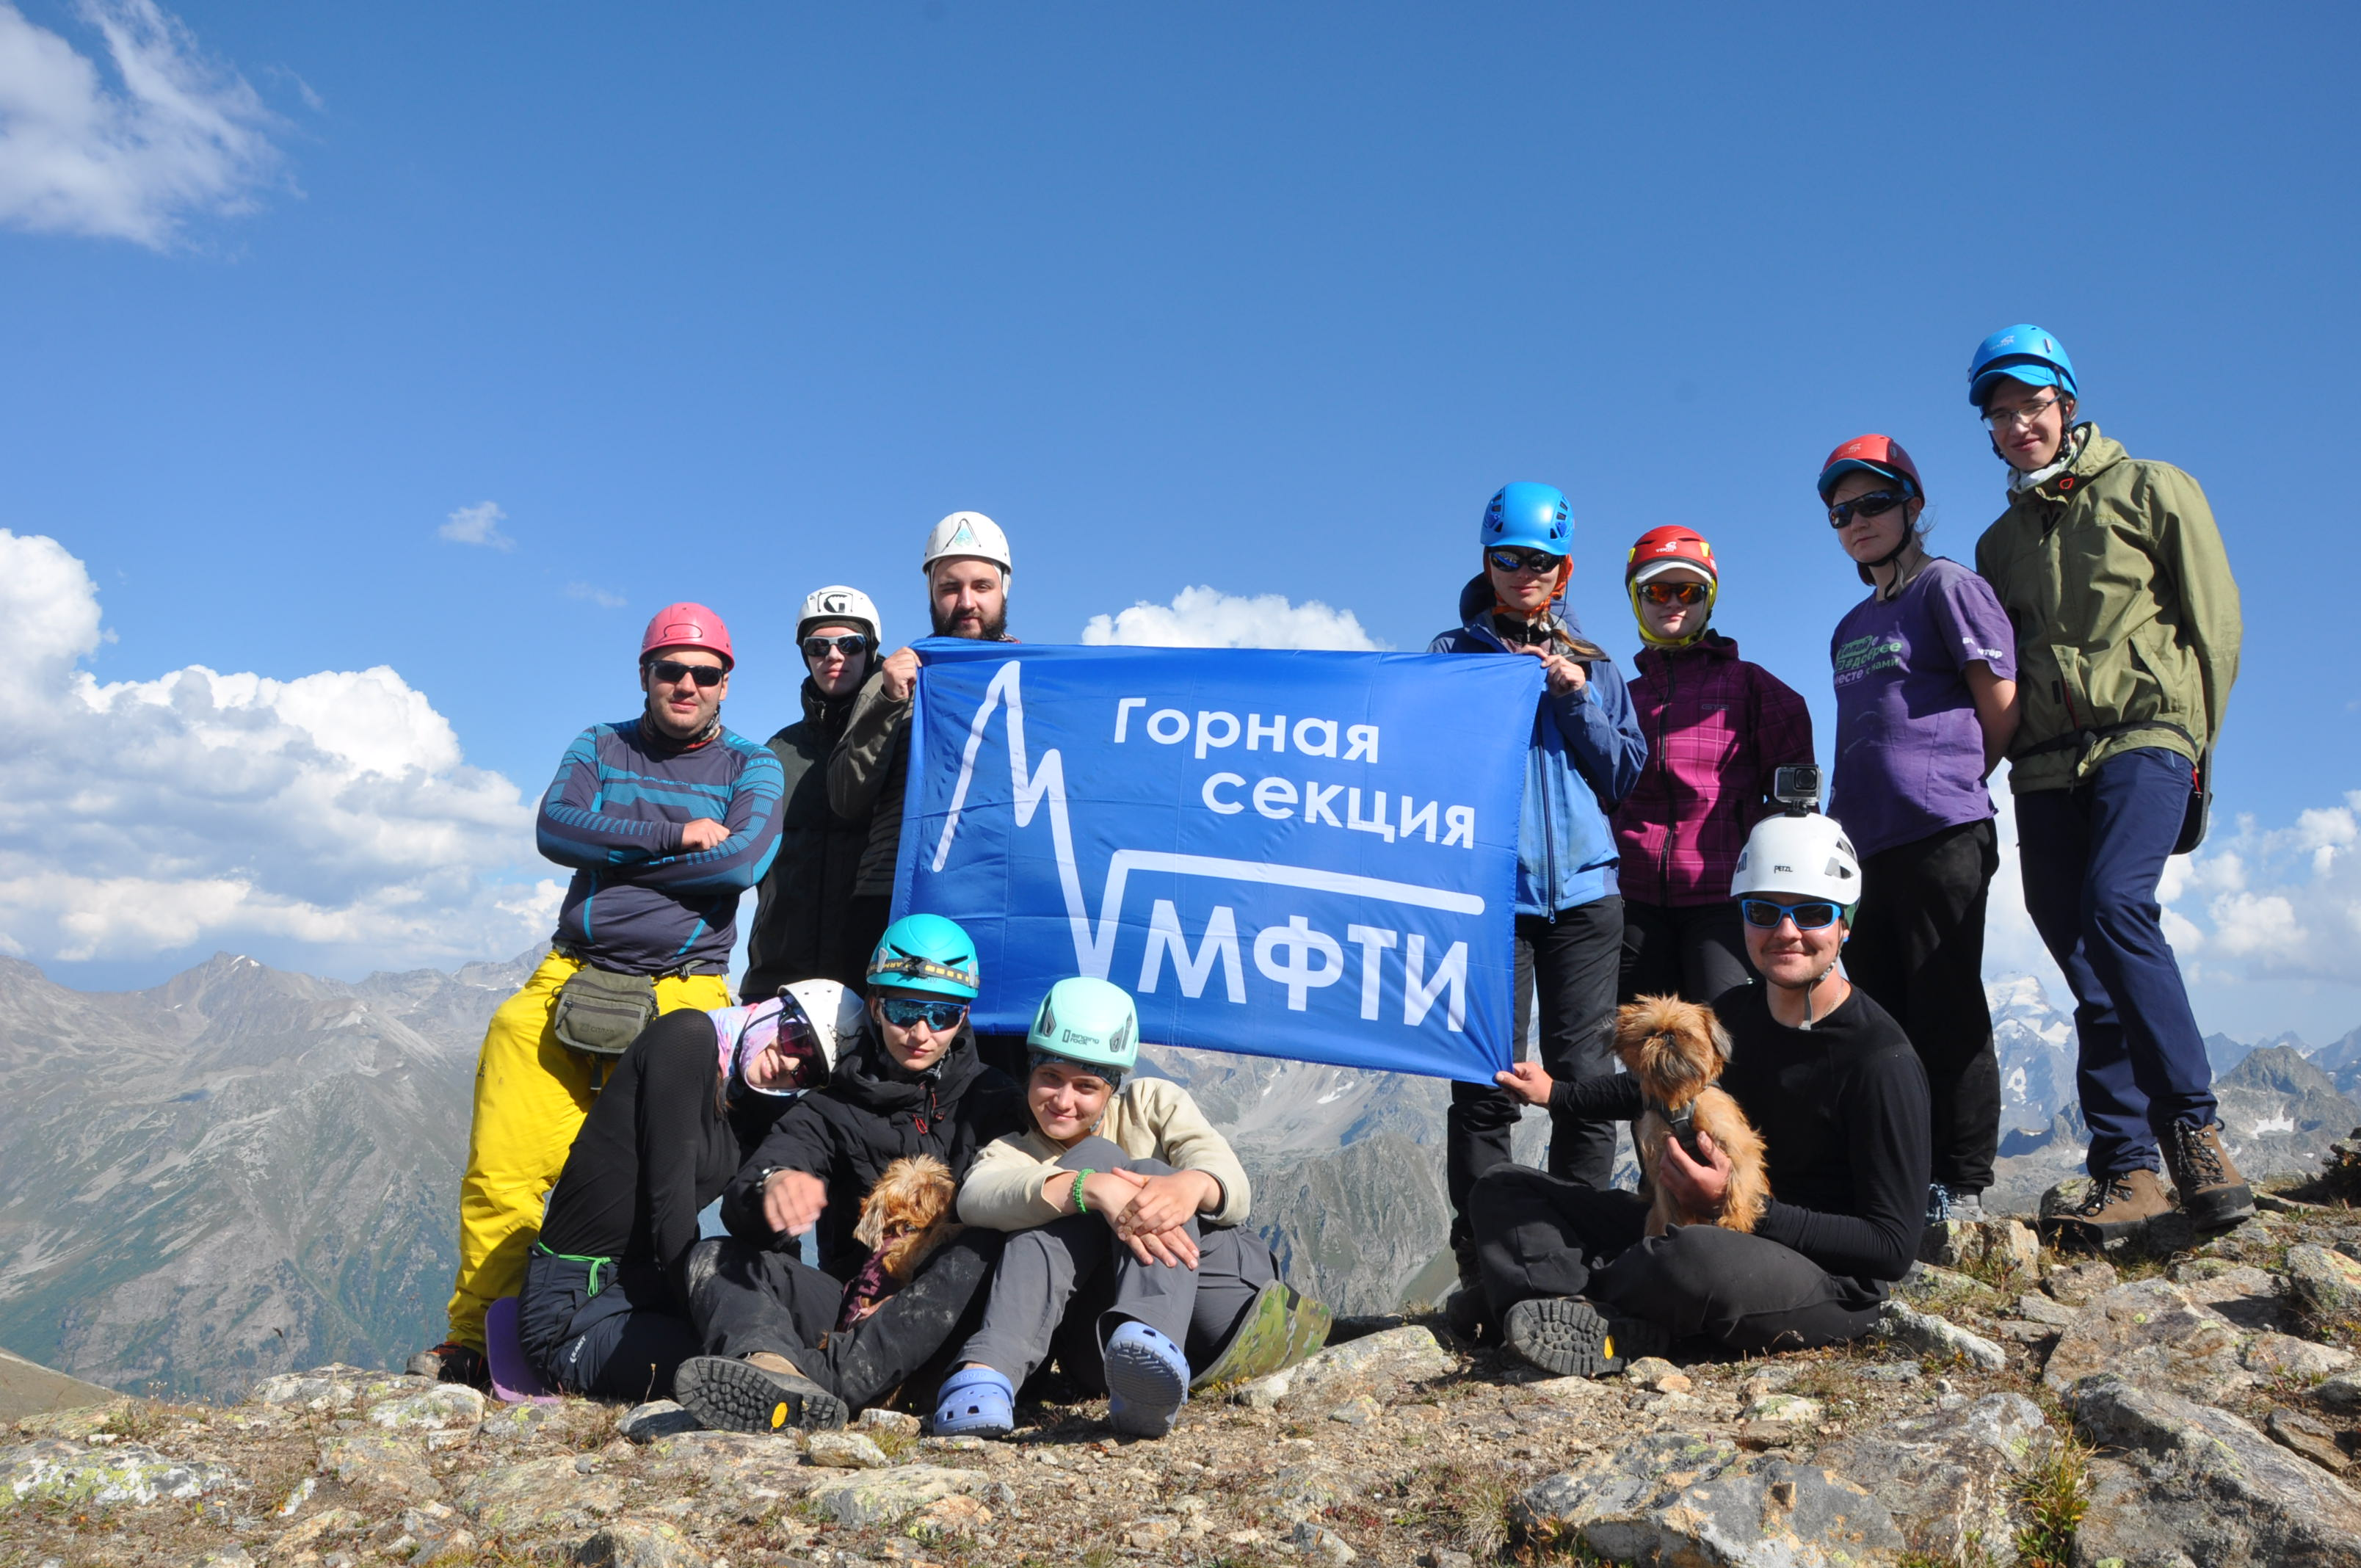
\includegraphics[width=0.7\linewidth]{../pics/DSC_0982}
	\caption{Группа на перевале, вид на д.р. Махар}
	\label{fig:DSC_0982}
\end{figure}

\begin{figure}[h!]
	\centering
	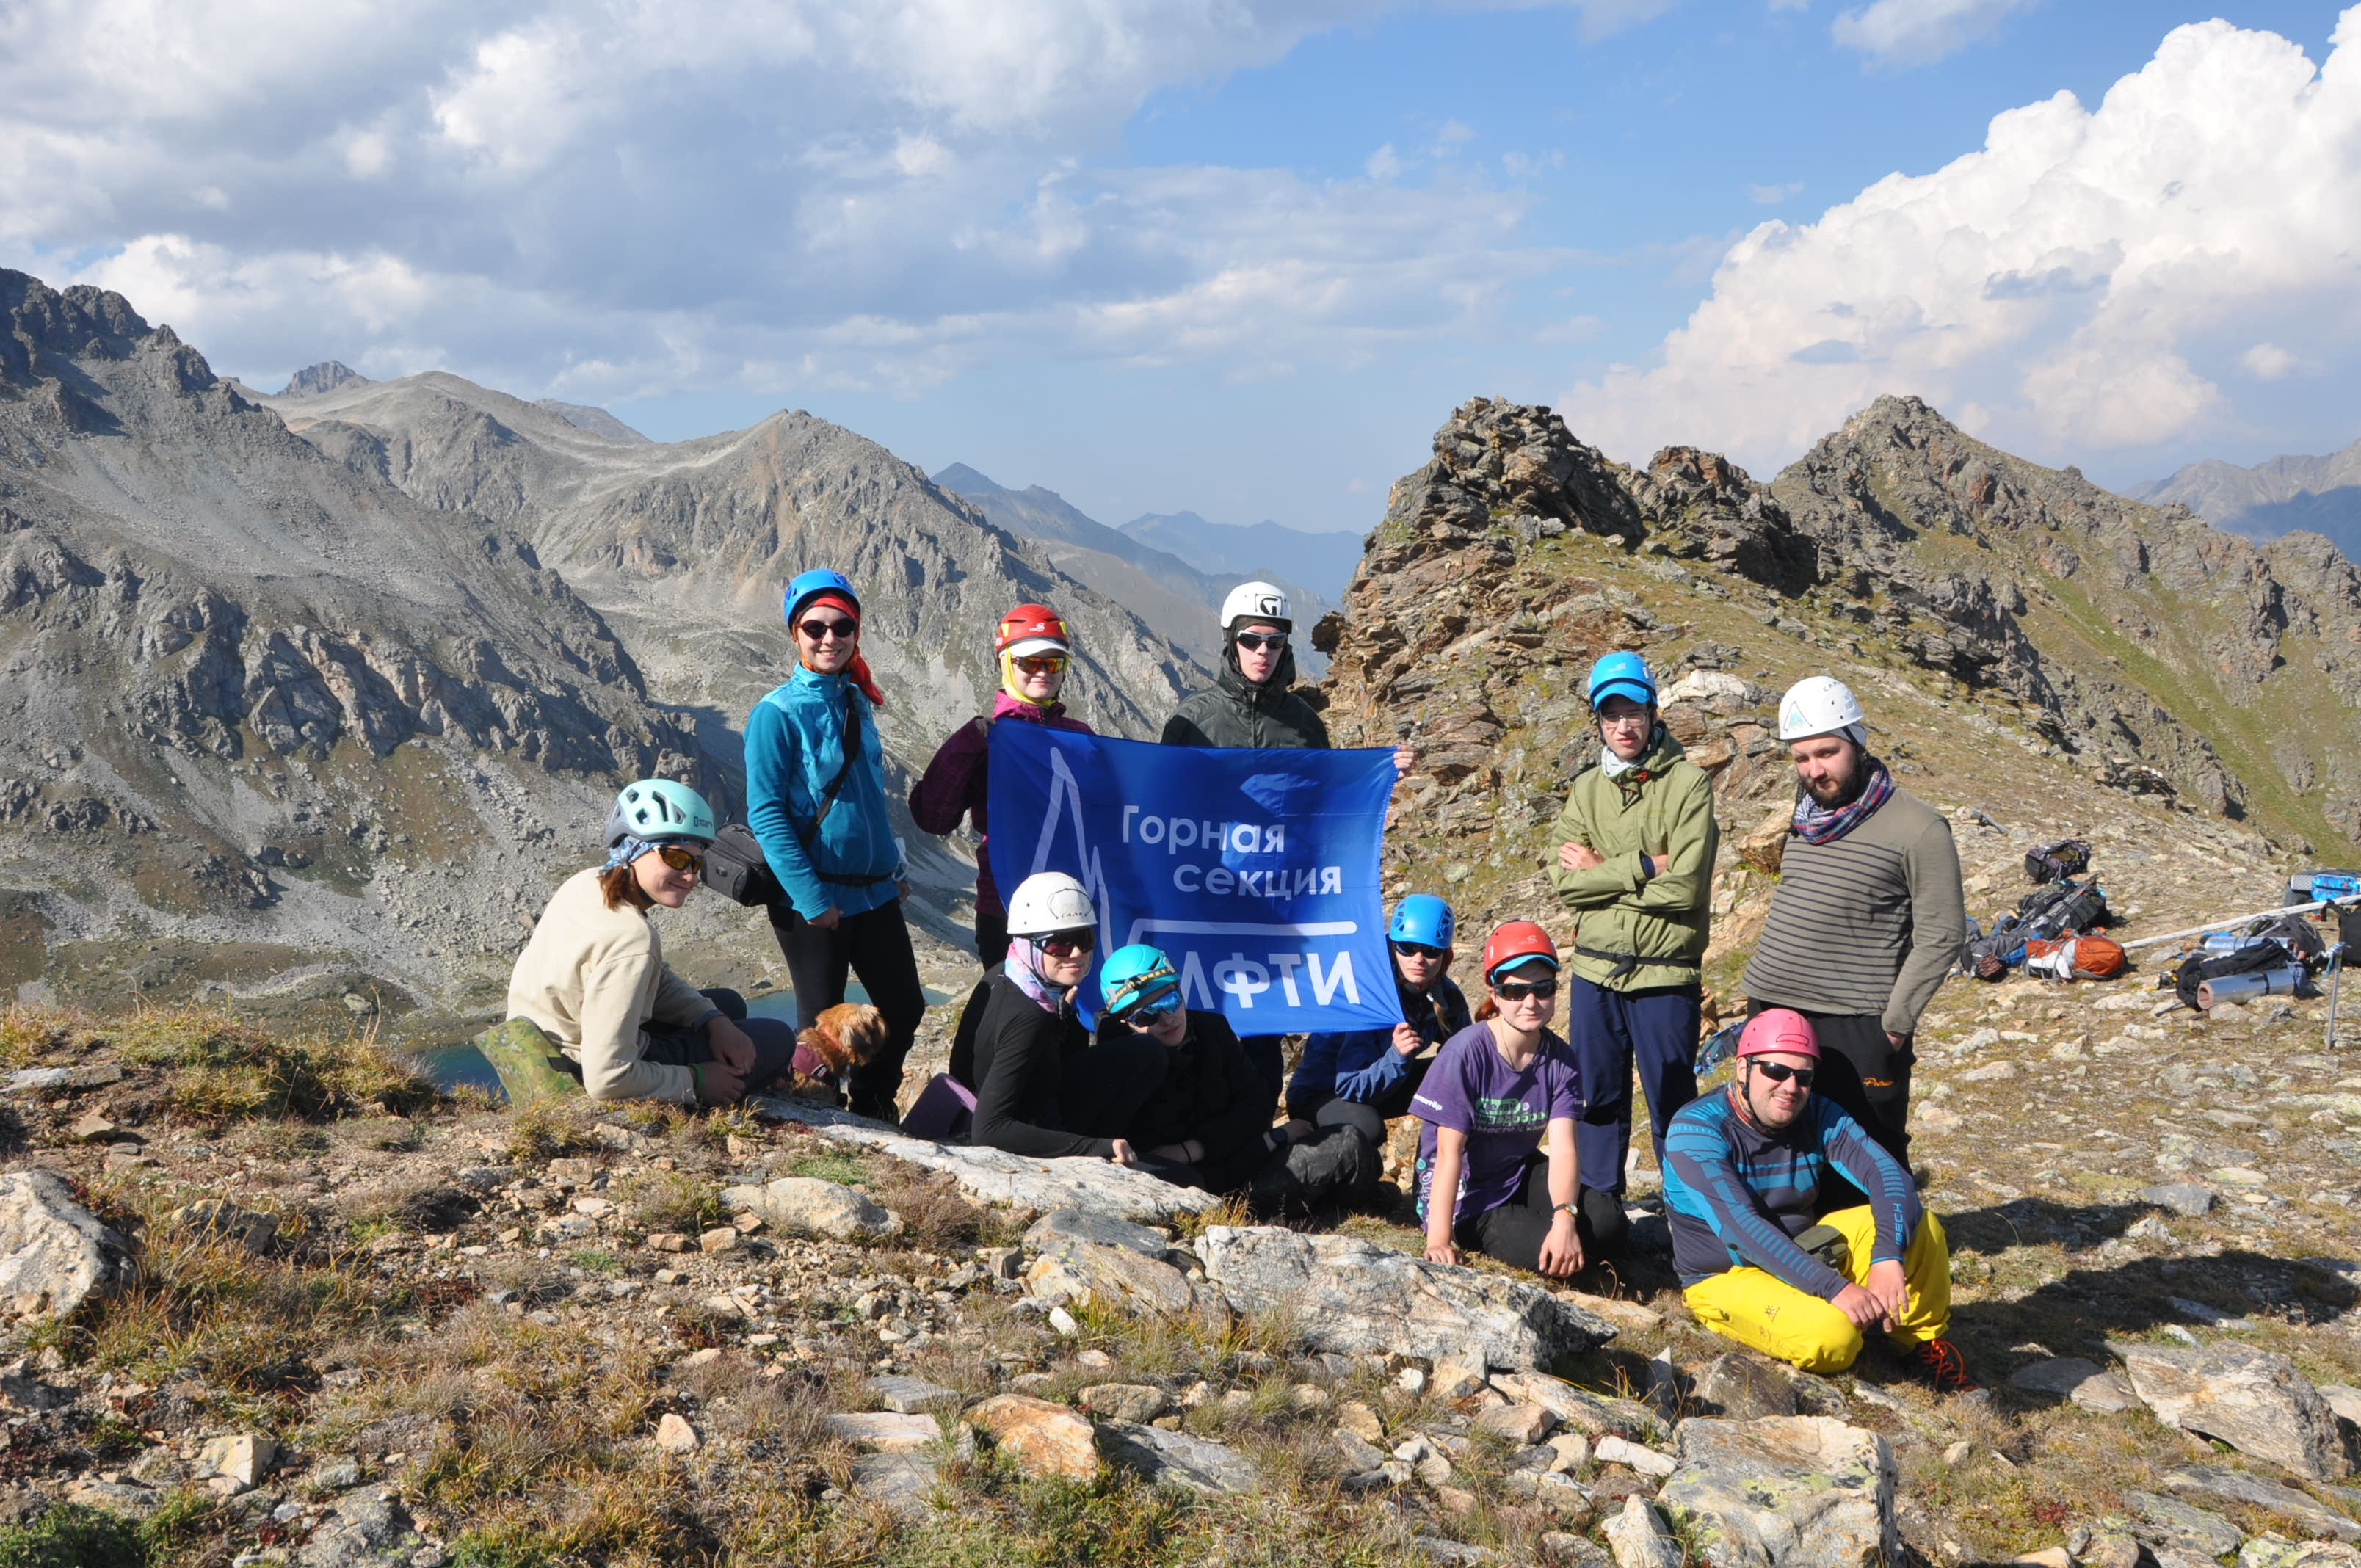
\includegraphics[width=0.7\linewidth]{../pics/DSC_0986}
	\caption{Группа на перевале, вид на оз. Уллу-Кёль}
	\label{fig:DSC_0986}
\end{figure}

\clearpage